\documentclass{article}
\usepackage[utf8]{inputenc}
\usepackage{algpseudocode}
\usepackage{algorithm}
\usepackage{tikz}
\usepackage{amsmath}
\usepackage{amssymb}
\usetikzlibrary{automata}
\setcounter{MaxMatrixCols}{25}

\title{Algorithmique Avancée TD02}
\author{Hugo Demaret}
\date{September 2021}
\begin{document}
\maketitle
\section*{Exercice 1.3 -}
\textit{Montrez que tout groupe d'au moins deux personnes contient toujours au moins deux individus ayant le même nombre d'amis.}\\
\textsf{Cas trivial du groupe à deux personnes :}\\
\textsf{Si connexe : 1 ami, sinon 0}\\
\textsf{Le graphe possède n sommet, et k arêtes.}\\
\textsf{On procède par récurrence :}
    \begin{center}
            On utilise le lemme des tiroirs :
            \linebreak
            On a n sommet, et au plus n-1 étiquette.
            \linebreak
            Par principe des tiroirs, au moins deux sommets on la même etiquette.
    \end{center}
\section*{Exercice 1.4 -}
    \textit{Soit $(d_{1},...,d_{n})$ la suite des degrés d'un graphe non-dirigé G.}\\
    \textit{On note $\delta(G)$ et $\bigtriangleup(G)$ respectivement le plus petit et le plus grand de ces sommets.}\\
    \subsection*{1 -}
        \textit{Montrez que $\sum_{i=1}^{n} di = 2m(G) $.}
            \begin{center}
            $
            \textit{Quand on ajoute une arête, on augmente le degré de deux sommets.}
            \linebreak
            \textit{La somme des degrés du graphe vaut n, et deux fois plus de sommets. D'ou :}
            \linebreak
            \sum_{i=1}^{n} di = 2m(G) 
            $
            \end{center}
    \subsection*{2 -}
            \textit{En déduire que $\delta(G) \leq \frac{2m(G)}{n(G)} \leq \bigtriangleup(G)$}\\
            \begin{center}
            $
            \forall i \in \{1,...,n\}, \delta(G) \leq d_{i} \leq \bigtriangleup(G)
            \linebreak
            \Rightarrow \sum_{i=1}^{n} \delta(G) \leq \sum_{i=1}^{n} d_{i} \leq \sum_{i=1}^{n} \bigtriangleup(G)
            \linebreak
            \Rightarrow n \delta(G) \leq 2m(G) \leq n\bigtriangleup(G)
            \linebreak
            \Rightarrow  \delta(G) \leq \frac{2m(G)}{n(G)} \leq \bigtriangleup(G)
            $
            \end{center}
\section*{Exercice 1.5 -}
\textit{Le but de cet exercice est de montrer que deux plus longs chemins dans un graphe\\ non-orienté connexe G ont forcément un sommet commun.}
    \subsection*{1 -}
            \subsubsection*{Démonstration 1 :}
            Si les deux chemins ont la même longueur :
            \linebreak
            - Soit ils partent du même sommet (ou arrivent au même) et sont joints.
            \linebreak
            - Soit ils ne partent pas du même sommet (et n'arrivent pas au même sommet).
            \linebreak
            On peut donc couper le graphe en deux sous graphes
            \linebreak
            Pour chacun de ces deux sous graphes, on ne considère que les chemins.
            \linebreak
            Ces sous graphes sont alors homéomorphe à un segment.
            \linebreak
            La distance étant égale, on peut tracer deux cordes
            \linebreak
            (les deux chemins) sur un cercle de rayon k, avec k étant le nombre de sommets
            \linebreak
            Ces deux cordes sont en fait des rayons, car de longueur k.
            \linebreak
            Deux rayons d'un cercle s'intersectent toujours.
            \linebreak
            Donc les deux chemins se croisent. Absurde.
        \subsubsection*{Démonstration 2 :}
            \textit{On essaie de représenter ce à quoi pourrait ressembler un tel graphe.}
            \textit{On montrera ensuite pourquoi un tel graphe, s'il existe, contedit les prémices de notre raisonnement.}
            \linebreak
            On suppose qu'il existe un graphe G simple et connexe, tel qu'il existe (au moins) deux chemins $\lambda$ et $\delta$ avec :
            $
            \lambda \cap \delta = \varnothing
            $
            Voici un schéma représentant ce graphe :
            \begin{center}
                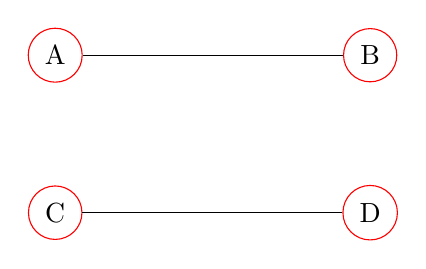
\begin{tikzpicture}
                    \node[circle,draw=red](A) at (0,0){A};
                    \node[circle,draw=red](B) at (4,0){B};
                    \node[circle,draw=red](C) at (0,-2){C};
                    \node[circle,draw=red](D) at (4,-2){D};
                    \draw[](A)--(B);
                    \draw[](C)--(D);
                \end{tikzpicture}
            \end{center}
            Ces deux chemins $(A,B)$ et $(C,D)$ sont de taille égale.
            Le graphe étant connexe, il existe un chemin $(\omega,\sigma)$ les reliants.
            Représentation :
            \begin{center}
                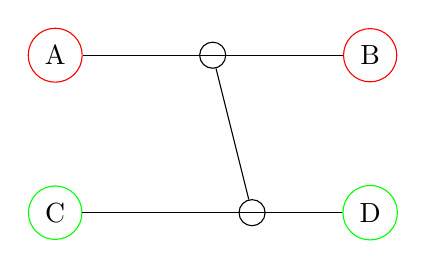
\begin{tikzpicture}
                    \node[circle,draw=red](A) at (0,0){A};
                    \node[circle,draw=red](B) at (4,0){B};
                    \node[circle,draw=green](C) at (0,-2){C};
                    \node[circle,draw=green](D) at (4,-2){D};
                    \draw[](A)--(B);
                    \draw[](C)--(D);
                    \node[circle,draw=black](E) at (2,0){};
                    \node[circle,draw=black](F) at (2.5,-2){};
                    \draw[](E)--(F);
                \end{tikzpicture}
            \end{center}
            On remarque qu'en passant par ce nouveau chemin, la distance parcouru est plus grande.
            Ces deux chemins les plus grands ne sont donc pas les plus grands. Absurde.
            Ou alors, le graphe n'est pas connexe. Absurde.
            Donc deux plus longs chemins dans un graphe G ne sont pas disjoints.
            $\square $
    \subsection*{2 -}
        Étant donné que les deux chemins se croisent (car non-disjoints), il existe au moins un sommet en commun.
    \subsection*{3 -}
        Dans le cas d'un graphe non-connexe non : graphe composé de deux fois un même sous graphe.
        Dans le cas d'un graphe orienté faiblement connexe, cette propriété est fausse :
        \begin{center}
            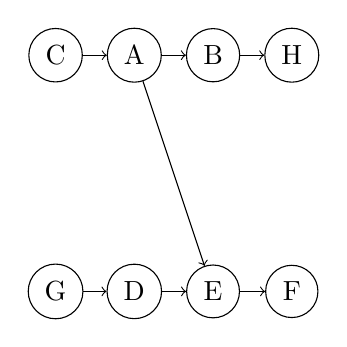
\begin{tikzpicture}
                \node[circle,draw=black](A) at(0,0) {A};
                \node[circle,draw=black](B) at (1,0) {B};
                \node[circle,draw=black](C) at (-1,0) {C};
                \node[circle,draw=black](H) at (2,0) {H};
                \node[circle,draw=black](D) at (0,-3) {D};
                \node[circle,draw=black](E) at (1,-3) {E};
                \node[circle,draw=black](F) at (2,-3) {F};
                \node[circle,draw=black](G) at (-1,-3) {G};
                \draw[->](C)--(A);
                \draw[->](A)--(B);
                \draw[->](B)--(H);
                \draw[->](E)--(F);
                \draw[->](D)--(E);
                \draw[->](G)--(D);
                \draw[->](A)--(E);
            \end{tikzpicture}
        \end{center}
    \section*{Exercice 1.6 -}
        Un graphe non-orienté est dit \textit{biparti} si $V(G)$ peut être partitionné en deux ensembles $A$ et $B$
        tels que toute arête de $G$ relie un sommet de $A$ et un sommet de $B$. On note $n(A)$ et $n(B)$ le nombre de sommets de $A$ et $B$.
        \subsection*{1 -}
            Le nombre maximal d'arêtes est donné de la façon suivante $n(A) \times n(B)$.
            La densité peut être définie comme suit :
            $$
            \frac{m(G)}{n(A)\times n(B)}
            $$
            \textit{Avec m(G) le nombre d'arêtes du graphe}
        \subsection*{2 -}
            Les sommets de $A$ alternent avec les sommets de $B$, et le dernier sommet est relié au premier, et par conséquent :
            
            \textit{Premier sommet noté s, dernier sommet noté d}
            $$
            \textit{si } s \in A, p \in B 
            $$
            Et réciproquement.\\
            Le nombre de sommet est donc forcément pair.
        \subsection*{3 -}
        On raisonne par l'absurde.
        Soient $p=2k$ et $g=2k+1$
        Alors pour le chemin $p$ $(u,v)$ appartient
    \section*{Exercice 1.7 -}
        \subsection*{1 -}
            Démonstration par récurrence :\\
            Soit $P_{k}$ la propriété est vrai au rang $k$\\
            $k=1$ est vraie (marche de longueur 1, donc présence de l'arête)\\
            Supposons la propriété vraie au rang k, k fixé. Montrons que cela entraine k+1.\\
            $$
                \left(M^{k+1}\right)_{u,v} = \sum_{w \in V(G)} \left(M^{k}\right)_{u,w} M_{w,v}
                = \sum_{w} \left(M^{k}\right)_{u,w}
            $$
            Avec $w$ qui est aussi un voisin de $v$\\\\
            Pour toute marche entre $u$ et $v$ de longueur $k+1$, il y a une marche de longueur $k$ entre $u$ et un voisin $w$ (réciproquement)\\
            La propriété est vraie au rang $1$ et $P(k) \Rightarrow P(k+1)$\\
            Donc la propriété est vraie par récurrence.\\\\
            \textit{En fait, on a une bijection entre les marches de longueur $k+1$ entre $(u,v)$\\ et les chemins de longueur $k$
            entre $(u,N(v))$}
            $\square$
        \subsection*{2 -}
            $M$ et $I$ sont commutantes (matrice identité)
            D'où :
            \begin{align*}
            \left(I+M\right)^{k} &= \sum_{k'=0}^{k} \binom{k}{k'}M^{k'}I^{k-k'}\\
            &= \sum_{k'=0}^{k} \binom{k}{k'}M^{k'}\\
            \end{align*}
            Tous les coefficients de cette somme sont positifs donc :
            $\left( \left(I+M\right)^{k} \right)_{u,v} > 0$
            ssi l'un des $M^{k'}$ est positif. $\square$
        \subsection*{3 -}
            S'il existe une marche entre $u$ et $v$ :
            On appelle cette marche P.
            Pour que P soit un chemin, P doit être la marche la plus courte (sans redondance).
            S'il y a une redondance ($i.e$ on passe au moins deux fois par le même sommet)
            alors ce n'est plus le plus court chemin. Il suffit donc de passer une seule fois par se sommet
            pour avoir un chemin.
            Donc s'il existe une marche entre $u$ et $v$, il existe un chemin $(u,v)$
            $\square$
        \subsection*{4 -}
            G est connexe d'où :\\
            G connexe $\Leftrightarrow \forall (u,v),$ il y a une marche $(u,v)$\\
            G connexe $\Leftrightarrow \forall (u,v),$ il y a un chemin $(u,v)$\\
            G connexe $\Leftrightarrow \forall (u,v), \exists k' \le k$ tel que $\left(M^{k'}\right)_{u,v}>0$\\
            G connexe $\Leftrightarrow \forall (u,v), \left( \left(I+M\right)^{k} \right)_{u,v} > 0$
            $\square$
        \subsection*{5 -}
            La complexité asymptotique du produit de deux matrices est $\mathcal{O}(n^{2})$
            Il faut faire ce produit $n$ fois. La complexité est donc $\mathcal{O}(n^{3})$\\
            Ce n'est pas très efficace, on préférera donc utiliser $BFS$ ou $DFS$.
\end{document}